\chapter{Debugging} \label{debugging}
%====================================
\index{debugger}

\section{Prolog-style Tracing and Debugging}
%===========================
\index{high-level tracing} \index{tracing!Prolog Programs}
%
XSB supports a version of the Byrd four-port debugger for interactive
debugging and tracing of Prolog code.  In this release (\version), it
does not work very well when debugging code involving tabled
predicates~\footnote{The current version of XSB's Prolog debugger does
  not include exceptions as a debugging port.}.  If one only creeps
(see below), the tracing can provide some useful information.  For
programs that involve large amounts of tabling forest-view tracing can
be used (Section~\ref{sec:forest-trace}).
To turn on tracing, use {\tt trace/0}, {\tt trace/1}, or {\tt trace/2}.  To
turn tracing off, use {\tt notrace/0}.

\begin{description}
\repeatstandarditem{trace}{trace/0}
\standarditem{notrace}{notrace/0}

When tracing is on, the system will print a message each time a
predicate is:
\begin{enumerate} \index{debugger!ports}
\item initially entered (Call), 
\item successfully returned from (Exit), 
\item failed back into (Redo), and
\item completely failed out of (Fail).  
\end{enumerate}
When debugging interactively, a message may be printed and tracer
stopped and prompts for input.  (See the predicates {\tt show/1} and
{\tt leash/1} described below to modify what is traced and when the
user is prompted.)

In addition to single-step tracing, the user can set spy points to
influence how the tracing/debugging works.  A spy point is set using
{\tt spy/1}.  Spy points can be used to cause the system to enter the
tracer when a particular predicate is entered. Also the tracer allows
``leaping'' from spy point to spy point during the debugging process.
%
The debugger also has profiling capabilities, which can measure the cpu
time spent in each call. The cpu time is measured only down to 0.0001-th
of a second.
g
When the tracer prompts for input, the user may enter a return, or a single
character followed by a return, with the following meanings:
\bi
\index{trace!options}
\item{\tt c, <CR>}: {\em Creep}~ Causes the system to single-step to
  the next port (i.e.\ either the entry to a traced predicate called
  by the executed clause, or the success or failure exit from that
  clause).
\item{\tt a}: {\em Abort}~ \index{abort!trace facility} Causes execution to abort
  and control to return to the top level interpreter.
\item{\tt b}: {\em Break}~ Calls the evaluable predicate {\em break},
  thus invoking recursively a new incarnation of the system
  interpreter.  The command prompt at break level $n$ is
  \begin{center}
    {\tt $n$: \tt ?-}
  \end{center}
  The user may return to the previous break level by entering the system
  end-of-file character (e.g.\ {\tt ctrl-D}), or typing in the atom 
  {\tt end\_of\_file}; or to the top level interpreter by typing in
  {\tt abort}.
\item{\tt f}: {\em Fail}~ Causes execution to fail, thus transferring
  control to the Fail port of the current execution.
\item{\tt h}: {\em Help}~ Displays the table of debugging options.
\item{\tt l}: {\em Leap}~ Causes the system to resume running the
  program, only stopping when a spy-point is reached or the program
  terminates.  This allows the user to follow the execution at a
  higher level than exhaustive tracing.
\item{\tt n}: {\em Nodebug}~ Turns off debug mode.
\item{\tt r}: {\em Retry (fail)}~ Transfers to the Call port of the current
  goal.  Note, however, that side effects, such as database modifications
  etc., are not undone.
\item{\tt s}: {\em Skip}~ Causes tracing to be turned off for the entire
  execution of the procedure.  Thus, nothing is seen until control comes
  back to that procedure, either at the Success or the Failure port.
\item{\tt q}: {\em Quasi-skip} This is like Skip except that it does not mask
  out spy points.
\item{\tt S}: {\em Verbose skip}~ Similar to {\tt Skip} mode, but trace
  continues to be printed. The user is prompted again when the current call
  terminates with success or failure.  This can be used to obtain a full
  trace to the point where an error occurred or for code profiling. (See
  more about profiling below.)
\item{\tt e}: {\em Exit}~ Causes immediate exit from \ourprolog\ back to the
  operating system.
\ei
%/* TLS: it seems like there may not be much use for the non-queryable trace/1 */

\standarditem{trace(+Filename,+option)}{trace/2}
\index{trace!logging}
%\index[pred]{\texttt{trace/1}}
%\index{\texttt{trace/1}}
%
{\tt trace/2} is like {\tt trace/0} except that it is non-interactive
and dumps trace information into a log file, {\tt Filename}.
Currently the only supported option is \texttt{log}.  However, the log
is written in the form of Prolog facts, which can be loaded
queried. The format of the facts is:
%% 
\begin{verbatim}
xsb_tracelog(CallId,CallNum,PortType,ParentCallNum,DepthOfCall,CurrentCall,Time)
\end{verbatim}
%% 
where \texttt{CallId} is an identifier generated when XSB encounters a
new top-level call. This identifier remains the same for all subgoals
called while tracing that top-level call.
\bi
\item \texttt{CallNum} is a generated number to show the nesting of
  the calls being traced. It is the same number that the user sees
  when tracing interactively.
%
\item \texttt{PortType} is \texttt{'Call'}, \texttt{'Redo'},
  \texttt{'Exit'}, or \texttt{'Fail'}.  
\item \texttt{ParentCallNum} is the call number of the parent call.
%
\item \texttt{DepthOfCall} is the nesting depth of the current call
  with respect to its ancestor calls.  
%
\item \texttt{CurrentCall} is the call being traced
%
\item \texttt{Time} is the CPU time it took to execute
  \texttt{CurrentCall}. On \texttt{'Call'} and \texttt{'Redo'},
  \texttt{Time} is always 0 --- it has a meaningful value only for the
  \texttt{'Exit'} and \texttt{'Fail'} log entries. 
\end{itemize}
It should be noted that when calls are delayed due to the well-founded
negation computation of because of the \texttt{when/2} primitive, the
parent call might be off in some cases. However, the parent property
repairs itself for subsequent calls.

`The name of the predicate (\texttt{xsb\_tracelog}) used for logging
can be changed by asserting it into the predicate
\texttt{debug\_tracelog\_predicate/1}, which should be imported from
\texttt{usermod}. For instance,
%% 
\begin{verbatim}
   :- import debug_tracelog_predicate/1 from usermod.
   ?- assert(debug_tracelog_predicate(foobar)).
\end{verbatim}
%% 

\standarditem{spy(Preds)}{spy/1}
    where {\tt Preds} is a spy specification or a list of such
    specifications, and must be instantiated. This predicate sets spy
    points (conditional or unconditional) on predicates.  A spy
    specification can be of several forms. Most simply, it is a term
    of the form $P$/$N$, where $P$ is a predicate name and $N$ its
    arity.  Optionally, only a predicate name can be provided, in
    which case it refers to all predicates of any arity currently
    defined in {\tt usermod}.  It may optionally may be prefixed by a
    module name, e.g.  $ModName$:$P$/$N$. (Again, if the arity is
    omitted, the specification refers to all predicates of any arity
    with the given name currently defined in the given module.)  A spy
    specification may also indicate a conditional spy point. A
    conditional spy specification is a Prolog rule, the head
    indicating the predicate to spy, and the body indicating
    conditions under which to spy. For example, to spy the predicate
    p/2 when the first argument is not a variable, one would write:
    $spy (p(X,\_):-nonvar(X)).$ (Notice that the parentheses around
    the rule are necessary). The body may be empty, i.e., the rule may
    just be a fact.  The head of a rule may also be prefixed (using
    $:$) with a module name. One should not put both conditional and
    unconditional spy points on the same predicate.

\standarditem{nospy(Preds)}{nospy/1}
    where {\tt Preds} is a spy specification, or a list of such
    specifications, and must be instantiated at the time of call.  What
    constitutes a spy specification is described above under {\tt spy}.
    {\tt nospy} removes spy points on the specified predicates. If a
    specification is given in the form of a fact, all conditional spy points
    whose heads match that fact are removed.

\standarditem{debug}{debug/0}
    Turns on debugging mode.
    This causes subsequent execution of predicates with trace or spy
    points to be traced, and is a no-op if there are no such predicates.
    The predicates {\tt trace/0}, {\tt trace/1}, \texttt{trace/2},  and {\tt spy/1} cause debugging mode
    to be turned on automatically.

\standarditem{nodebug}{nodebug/0}
    Turns off debugging mode.  This causes trace and spy points to be ignored.

\standarditem{debugging}{debugging/0}
    Displays information about whether debug mode is on or not, and lists
    predicates that have trace points or spy points set on them.

\standarditem{debug\_ctl(option,value)}{debug\_ctl/2}
   {\tt debug\_ctl/2} performs debugger control functions as described below.
   These commands can be entered before starting a trace or inside the trace.
   The latter can be done by responding with ``{\tt b}'' at the prompt,
   which recursively invokes an XSB sub-session. At this point, you can
   enter the debugger control commands and type \verb|end_of_file.| This
   returns XSB back to the debugger prompt, but with new settings.
   %%
   \begin{enumerate}
   \item {\tt debug\_ctl(prompt, off)} Set non-interactive mode globally.
     This means that trace will be printed from start to end, and the user
     will never be prompted during the trace.
    \item {\tt debug\_ctl(prompt, on)} 
      Make tracing/spying interactive.
    \item {\tt debug\_ctl(profile, on)}  
      Turns profiling on. This means that each time a call execution
      reaches the {\tt Fail} or {\tt Exit} port, CPU time spent in that
      call will be printed. The actual call can be identified by locating a
      {\tt Call}  prompt that has the same number as the ``cpu time''
      message.
    \item {\tt debug\_ctl(profile, off)}  
      Turns profiling off.
    \item {\tt debug\_ctl(redirect, +File)} 
      Redirects debugging output to a file. This also includes program output,
      errors and warnings.
      Note that usually you cannot see the contents of {\tt +File} until it
      is closed, {\it i.e.}, until another redirect operation is performed
      (usually {\tt debug\_ctl(redirect, tty)}, see next).
    \item {\tt debug\_ctl(redirect, tty)}     
      Attaches the previously redirected debugging, error, program output,
      and warning streams back to the user terminal.
    \item {\tt debug\_ctl(show, +PortList)}  
      Allows the user to specify at which ports should trace messages be
      printed. {\tt PortList} must be a list of port names, i.e., a sublist
      of ['Call', 'Exit', 'Redo', 'Fail']. 
    \item {\tt debug\_ctl(leash, +PortList)}  
      Allows the user to specify at which ports the tracer should stop
      and prompt the user for direction.  {\tt PortList} must be a list of
      port names, i.e., a sublist of ['Call', 'Exit', 'Redo', 'Fail'].  Only
      ports that are {\tt show}-n can be {\tt leash}-ed. 
    \item {\tt debug\_ctl(hide, +PredArityPairList)}  
      The list must be of the form {\tt [P1/A1, P2/A2, ...]}, {\it i.e.},
      each either must specify a predicate-arity pair. Each predicate on
      the list will become non-traceable. That is, during the trace, each
      such predicate will be treated as an black-box procedure, and trace
      will not go into it.
    \item {\tt debug\_ctl(unhide, ?PredArityPairList)} If the list is a
      predicate-arity list, every predicate on that list will become
      traceable again. Items in the list can contain variables. For
      instance, {\tt debug\_ctl(unhide, [\_/2])} will make all 2-ary that
      were previously made untraceable traceable again.  As a special case,
      if {\tt PredArityPairList} is a variable, all predicates previously
      placed on the ``untraceable''-list will be taken off.
    \item {\tt debug\_ctl(hidden, -List)}
      This returns the list of predicates that the user said should not be
      traced.
   \end{enumerate}
   %%
\end{description}


\section{Low-Level Tracing}
%--------------------------------------------------
\index{low-level tracing} \index{tracing!low-level}

XSB also provides a facility for low-level tracing of execution.  This
can be activated by invoking the emulator with the {\tt -T} option
(see Section~\ref{sec:EmuOptions}), or through the predicate {\tt
  trace/0}.  \stdrefindex{\$trace/0} It causes trace information to
be printed out at every call (including those to system trap
handlers).  The volume of such trace information can very become large
very quickly, so this method of tracing is not recommended in general.

\bigskip

XSB debugger also provides means for the low-level control of what
must be traced. Normally, various standard predicates are masked out
from the trace, since these predicates do not make sense to the
application programmer.  However, if tracing below the application
level is needed, you can retract some of the facts specified in the
file {\tt syslib/debugger\_data.P} (and in some cases assert into
them). All these predicates are documented in the header of that
file. Here we only mention the four predicates that an XSB developer
is more likely to need. To get more trace, you should retract from the
first three predicates and assert into the last one.
%%
\begin{itemize}
\item {\tt hide\_this\_show(Pred,Arity)}: specifies calls (predicate name and
  arity) that the debugger should {\tt not} show at the prompt. However,
  the evaluation of this hidden call {\tt is} traced.
\item {\tt hide\_this\_hide(Pred,Arity)}: specifies calls to hide. Trace
  remains off while evaluating those predicates. Once trace is off, there
  is no way to resume it until the hidden predicate exits or fails.
\item  {\tt show\_this\_hide(Pred,Arity)}: calls to show at the
  prompt. However, trace is switched off right after that.
\item  {\tt trace\_standard\_predicate(Pred,Arity)}: Normally trace doesn't
  go inside standard predicates ({\it i.e.}, those specified in
  {\tt syslib/std\_xsb.P}. If you need to trace some of those, you must
  {\tt assert} into this predicate.
\end{itemize}
%%
In principle, by retracting all facts from the first three predicates and
asserting enough facts into the last one, it is possible to achieve the
behavior that approximates the {\tt -T} option. However, unlike {\tt -T},
debugging can be done interactively. This does not obviate {\tt -T},
however. First, it is easier to use {\tt -T} than to issue multiple asserts
and retracts. Second, {\tt -T} can be used when the error occurs early on,
before the moment when XSB shows its first prompt.

%-----------------------------------------------------------------------------
\newcommand{\mif}{\mbox{ :- }}
\newcommand{\cS}{{\cal S}}
\newcommand{\ctrace}{{\tt logforest}}

\section{Analyzing the Execution of Tabled Programs} \label{sec:forest-trace}
%
The sort of tracing and debugging described in previous sections has
proven useful for Prolog programs for 30 or more years.  However, when
tabling is added to Prolog, things change.  First, as described in
Chapter~\ref{chap:TablingOverview}, tabling can be used to find the
least fixed point of mutually recursive predicates.  Operationally,
this requires the ability to suspend one computation path and to
resume another.  The addition of tabled negation for the well-founded
semantics also requires the ability to delay negative goals whose only
proof may be involved in a loop through negation and to simplify these
goals once their truth value has become known. Furthermore, a tabled
subgoal has different states: it may be {\em new}; it may be {\em
  incomplete} so that new answers might be derived for it; or {\em
  completed} so that the answers may simply be read from the table.
In short, tabling, which can execute much more general programs than
Prolog and can use the stronger well-founded semantics, requires a
more complex set of operations than Prolog's SLDNF so that debugging
and tracing is correspondingly more complex.  Thus, while the 4-port
debugger may be useful for programs that involve just a few tabled
predicates, it may not be useful for programs that heavily use tabling
for complex recursions, non-monotinic reasoning or other purposes.

There is currently no standard approach to debugging tabled programs.
One possible approach would be to extend the 4-port debugger to
include other ports for tabling operations.  Such extensions have not
yet been explored, and whether the paradigm of n-port debugging can be
extended to full tabling so that it can be useful to programmers is an
open question.  Another approach would be use the declarative approach
of {\em justification} \cite{GuRR01,PGDRR04} to explain why
derivations were or were not made.  XSB does in fact have a
justification package but it is not currently robust enough to be
recommended for general use.  Below we present the {\tt \ctrace}
approach.

\subsection{Tracing a tabled evaluation through forest logging}
%
While the operations used for tabling are more complex than those of
SLDNF, they have a clear formal operational semantics through SLG and
the forest-of-trees model.  We recall this model briefly below for a
definite program but assume a background knowledge of tabled logic
programming (see, for instance~\cite{SwiW10}).

\begin{example} \rm 
Figure~\ref{fig:local} shows a program fragment along with an SLG
forest for the query {\tt ?- reach(1,Y)} to the the right-recursive
tabled predicate {\tt reach/1}.  An SLG forest consists of an SLG tree
for each tabled subgoal $S$: this tree has root $S \mif{} S$.  In a
definite program an SLG tree represents resolution of program clauses
and answers to prove $S$.  In Figure~\ref{fig:local} each non-root
node of the form $K. N$ where $N = (S \mif{} Goals)\theta$ is a clause
in which the bindings to a subgoal $S$ are maintained in $S\theta$,
the goals remaining to prove $S$ are in $Goals\theta$, and the order
of creation of $N$ within the tabled evaluation is represented by a
number, $K$ (local scheduling is used in this example).  Children of a
root node are obtained through resolution of a tabled subgoal against
program clauses.  Children of non-root nodes are obtained through
answer clause resolution, if the left most selected literal is tabled
(e.g. children of node 3 or 11 in the tree for {\tt reach(1,Y)}), or
through program clause resolution if the leftmost selected literal is
not tabled (e.g. children of nodes 2 and 18 in the tree for {\tt
  reach(1,Y)}).  Nodes that have empty {\em Goals} are termed {\em
  answers}.
%
\begin{figure}[htbp]
\centering
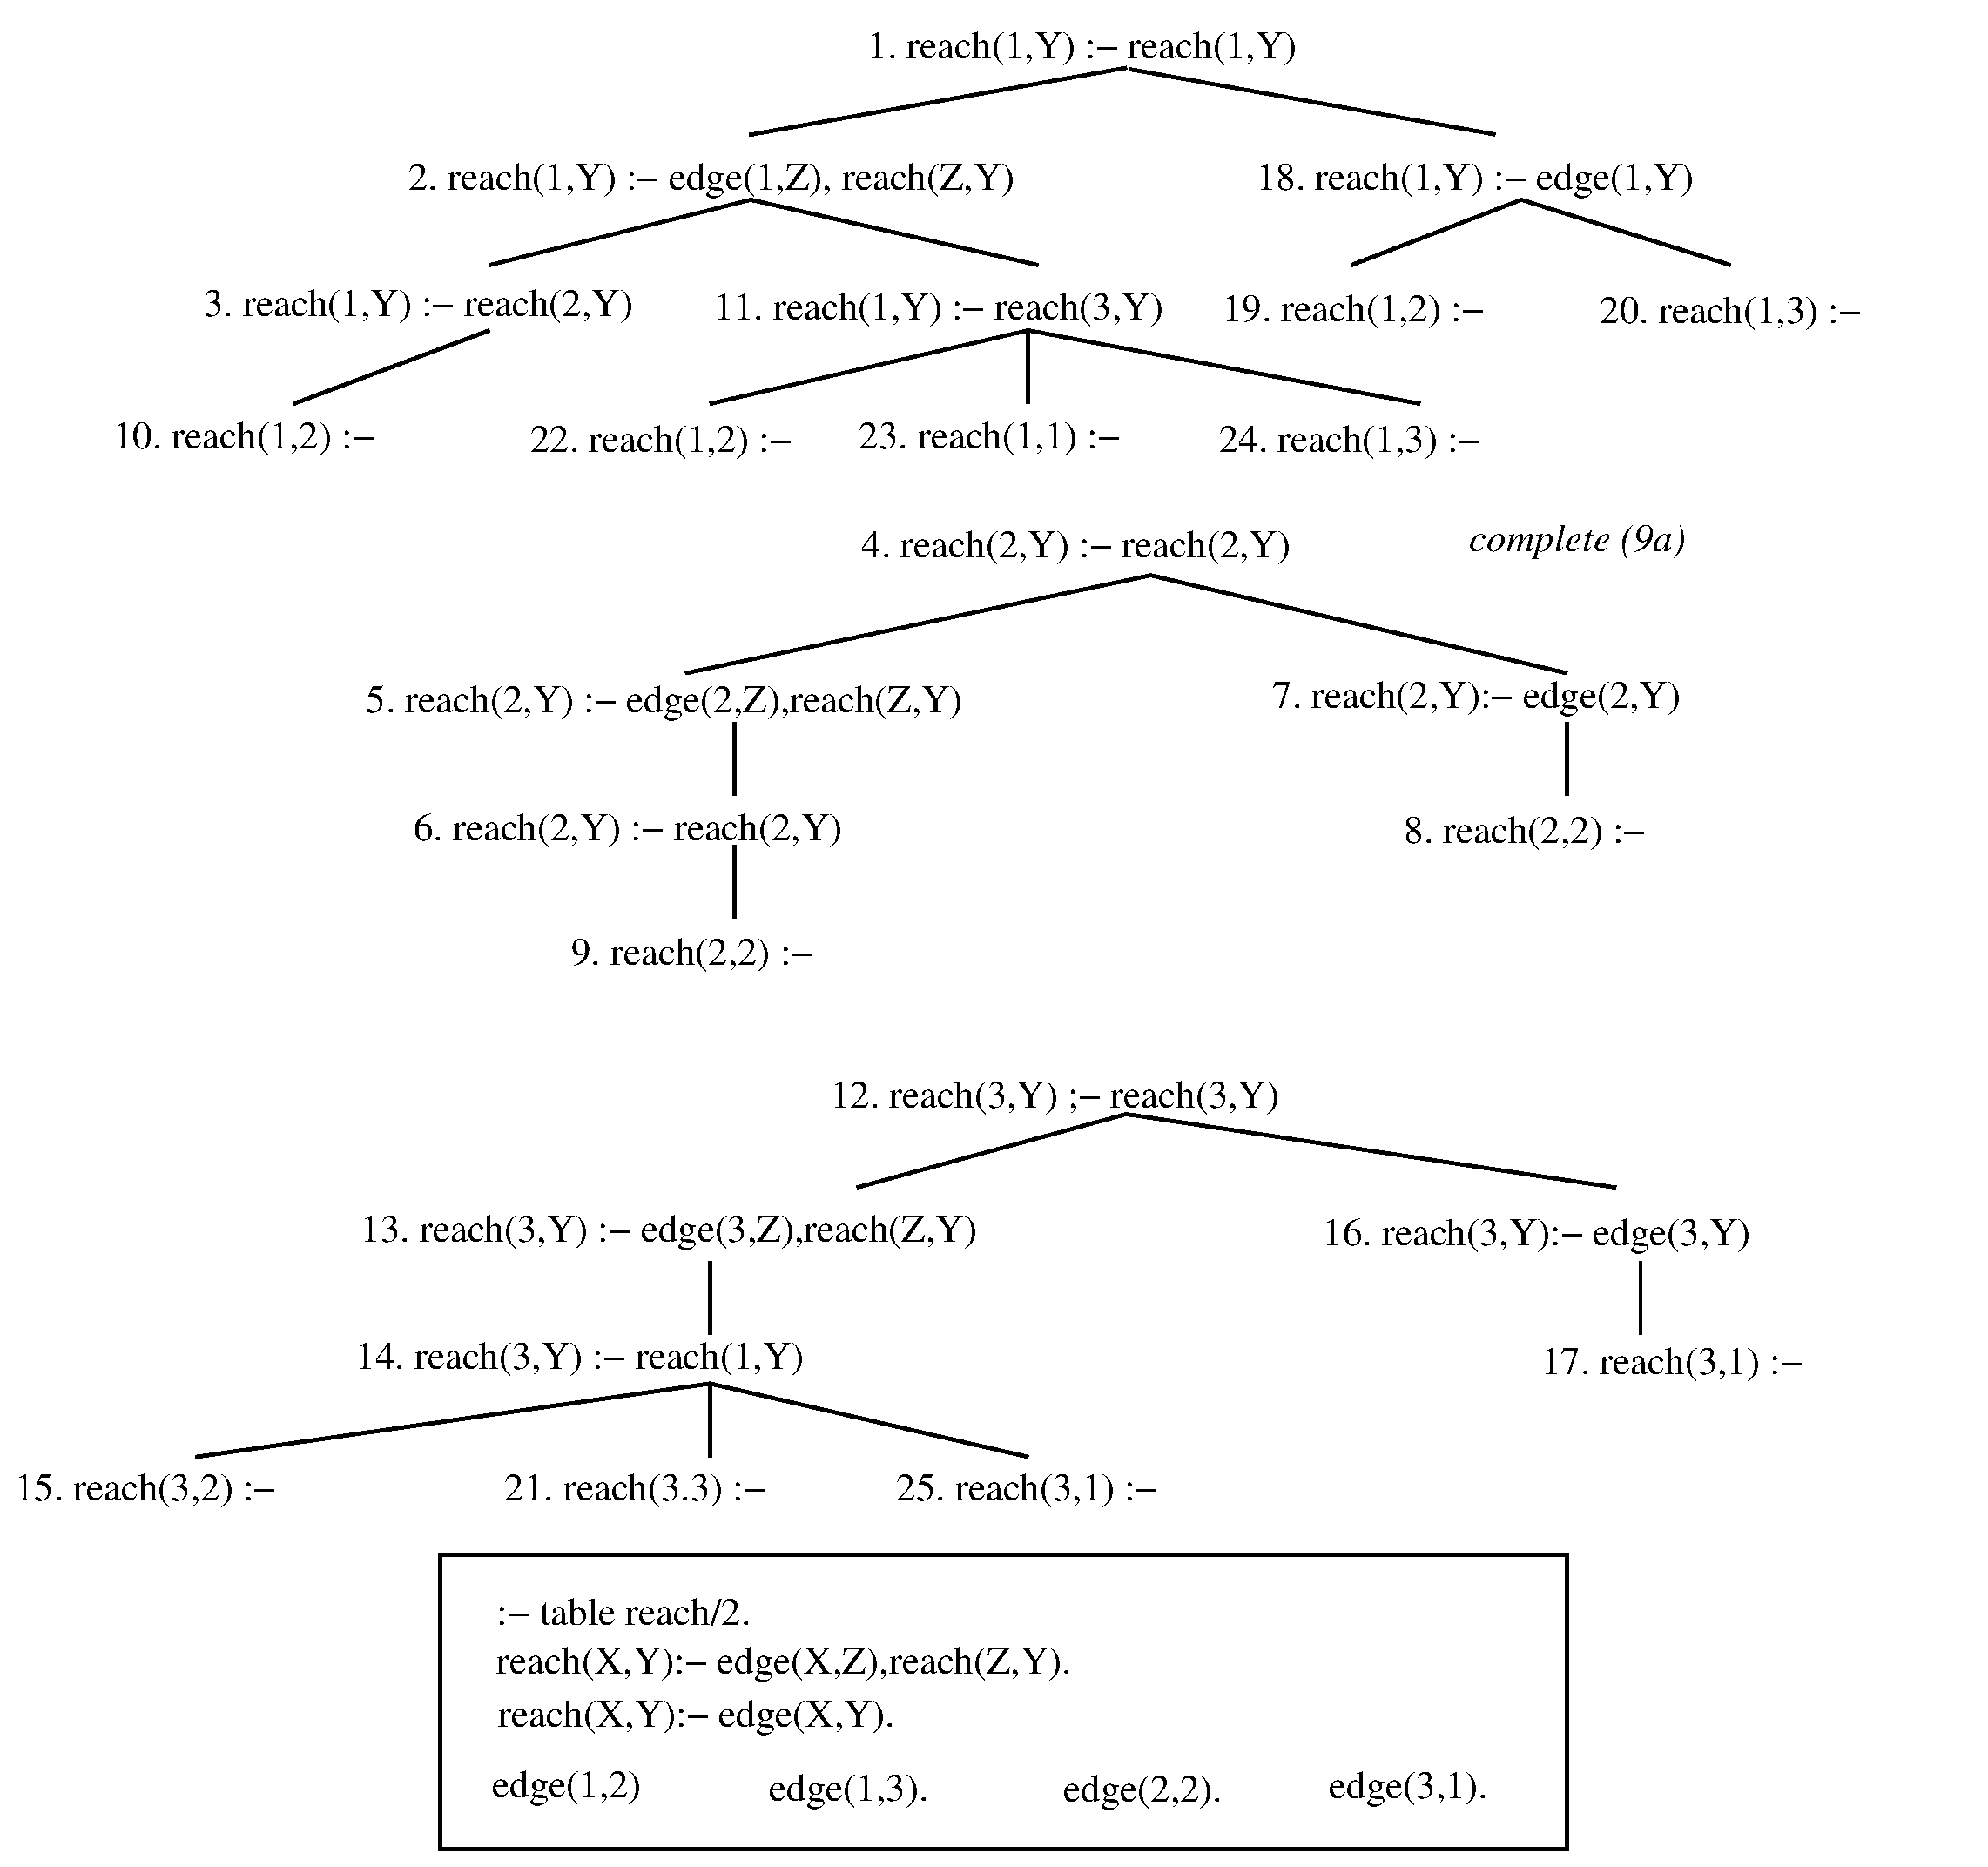
\includegraphics[width=.99\textwidth]{slg-forest-local}
%%\mbox{
%%{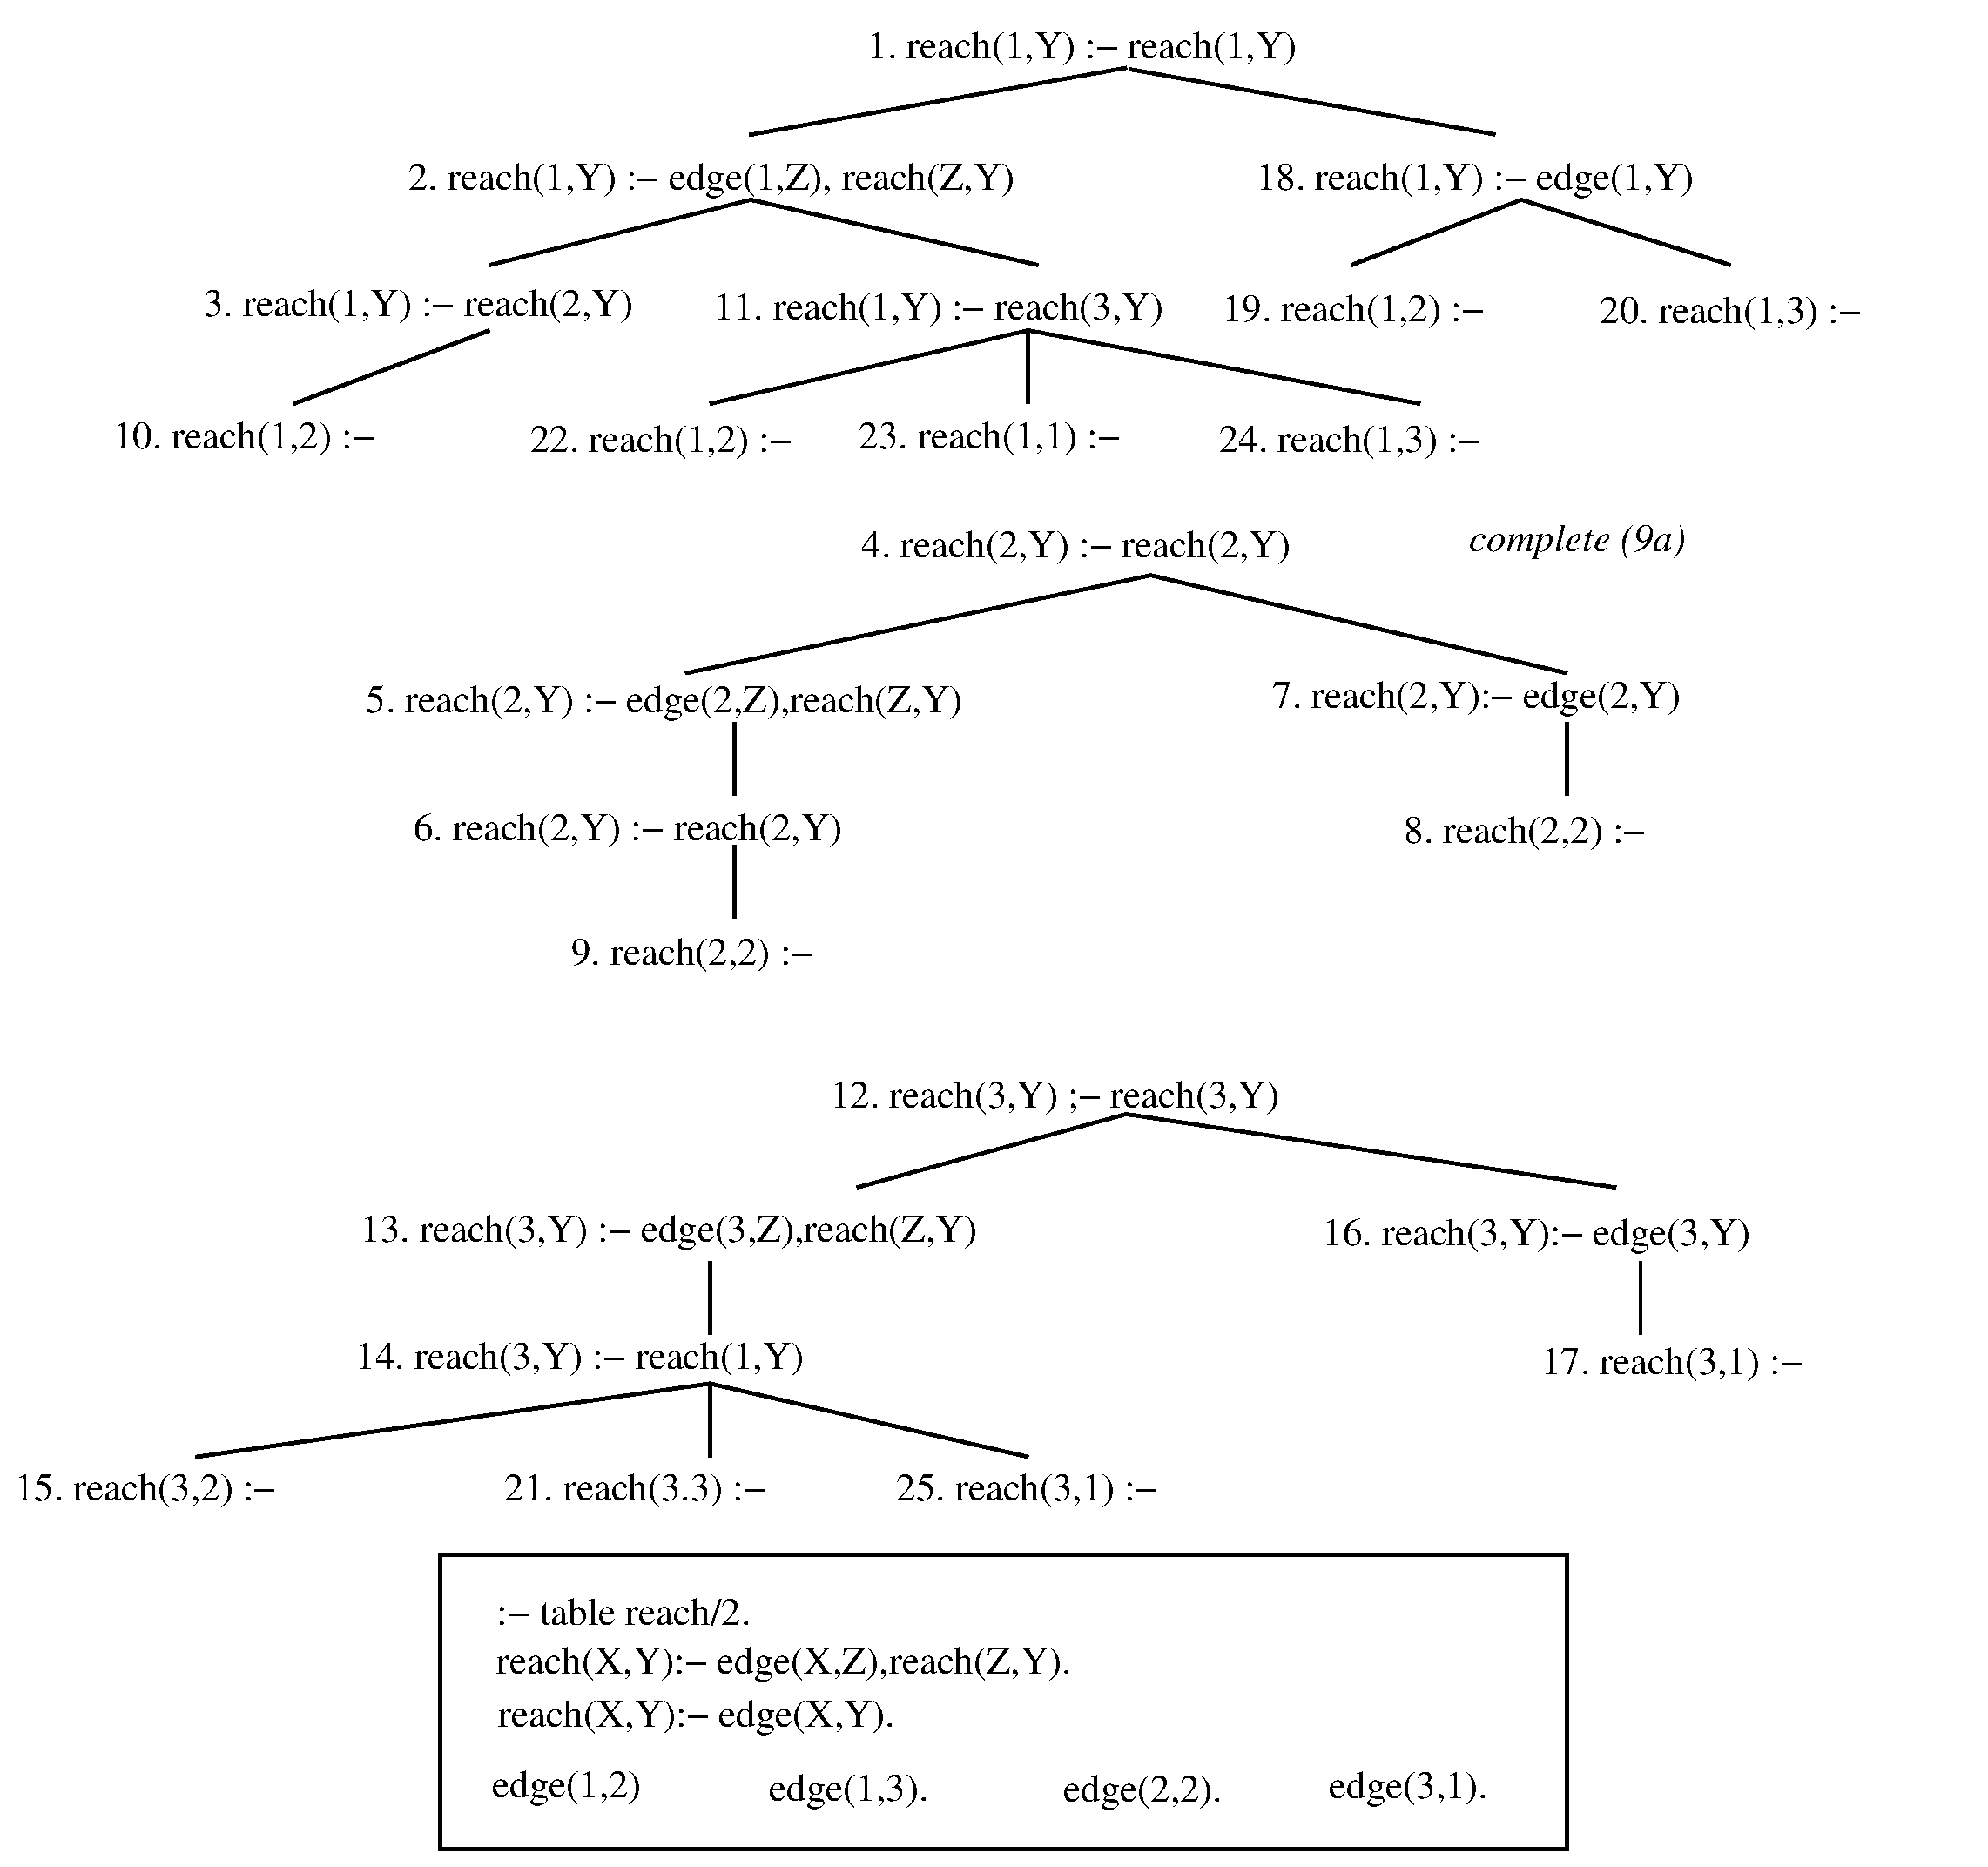
\epsfig{file=slg-forest-local,width=.99\textwidth}}}
\caption{A program $P_{Rrec}$ and SLG forest for (local) evaluation of
  {\tt ?- reach(1,Y)}} \label{fig:local}
\end{figure}
%
Note that the evaluation keeps track of each tabled subgoal $S$ that
it encounters.  Later if $S$ is selected again, resolution will use
answers rather than program clauses; if no answers are available, the
computation will {\em suspend} at that point and the evaluation will
backtrack to try to derive answers using some other computation path.
Once more answers have been derived, the evaluation {\em resumes} the
suspended computation.  Similarly, once the computation has
backtracked through all answers available for $S$ in the current
state, the computation path will suspend, and resume after further
answers are found.  Thus a tabled evaluation is a fixed point
computation for a set of interdependent subgoals.  When it is
etermined that a (perhaps singleton) set of subgoals can produce no
more answers, the subgoals are completed.
\end{example}

%\vspace{0.1in}

The forest logging approach ({\tt \ctrace}) allows one to run a tabled
query and produce a log that can be interpreted as (a partial image
of) an SLG forest.  The log can then used to analyze program
correctness, to optimize performance and so on.  Because \ctrace{}
  produces a log, it superficially resembles the non-interactive trace
  described earlier in this chapter.  However,
\begin{itemize}
\item {\tt trace/1} produces a Prolog-style trace that takes little
  account of tabling.  \ctrace{} structures its output according to
  the forest-of-trees model, and takes little account of program
  clause resolution.

\item \ctrace{} is implemented in C for efficiency, while {\tt
  trace/1} is built on top of XSBs interactive debugger.  Unlike {\tt
  trace/1}, \ctrace{} can therefore to produce logs for very large
  evaluations with little overhead.
\end{itemize}

{\em We stress that the forest logging approch is under development and
  its features are subject to change.}

Currently, \ctrace{} captures the following actions.

\bi
\item {\em A call to a tabled subgoal}~ If a call to a tabled subgoal
  $S_1$ is made from a tree for $S_2$ a Prolog-readable fact of the
  form {\tt tc(S1,S2,Stage,Counter)} is logged, where {\em Counter} is
  the ordinal number of the fact, and {\tt Stage} is
\bi
\item {\tt new} if $S_1$ is a new subgoal
\item {\tt cmp} if $S_1$ is not a new subgoal and has been completed
\item {\tt incmp} if $S_1$ is not a new subgoal but has {\em not} been
  completed \ei
%
  For instance, in the above example, node 3 would be represented as
  {\tt tc(reach(2,Y),reach(1,Y),2)} (the reason for using the counter
  value of 2 rather than 3 is explained below).  If $S_1$ is the first
  tabled subgoal in an evaluation, $S_2$ is the atom {\em null}.

\item {\em Derivation of a new answer}~ When a new answer $A$ is
  derived for subgoal $S$ and added to the table (i.e. $A$ is not
  already an answer for $S$) a fact of the form {\tt na(A,S,Counter)}
  is logged.  In the above example, the answer node 9 would be
  represented as {\tt na([2],reach(2,\_v1),4)} where the first argument
  is a list of substitutions for the variables {\em \_v1,...,\_vn} in
  $S$.

\item {\em Return of an answer to a consuming subgoal}~When an answer
  $A$ is returned to a consuming subgoal $S$ in a tree for $S_T$, a
  fact of the form {\tt ar(A,S,ST,Counter)} is logged.  A log entry is
  made only if the table for $S$ is incomplete (see the explanation
  below).

\item {\em Subgoal completion}
\bi
\item When a set $\cS$ of subgoals is determined to be completely
  evaluated and is completed, a fact of the form {\tt
    cmp(S,SCCNum,Counter)} is logged for each $S \in \cS$.  Here
  $SCCNum$ is simply a number giving an ordinal value that can be used
  to group subgoals into mutually dependent sets of subgoals or SCCs,
  i.e. the {\em SCCNum} of each $S \in \cS$ has the same value, but
  that value is not used for a completion fact of any subgoal not in
  $\cS$.
%
\item When a subgoal $\cS$ is {\em early completed}, i.e. it is
  determined that no more answers for $S$ are possile or are desired a
  fact of the form {\tt cmp(S,ec,Counter)} is logged.  If $S$ belonged
  to a larger mutually dependent set $\cS$ when it was early
  completed, $S$ will also be included in the completion facts for
  $\cS$.
\ei
\item {\em Table Abolishes}
\bi
\item When a tabled subgoal $S$ is abolished, a fact of the form {\tt
  ta(subg(S),Counter)} is logged.
\item When all tables for a predicate $p/n$ are abolished, a fact of
  the form {\tt ta(pred(p/n),Counter)} is logged.
\item When all tables are abolished, a fact of the form {\tt ta(all,Counter)} is logged.
\ei
%
\item {\em Location of errors} Whenever an error is thrown and the
  execution is in a tree for a subgoal $S$, a Prolog-readable fact of
  the form {\tt err(S,Counter)} is logged, where {\em Counter} is the
  ordinal number of the fact.  The primary purpose of this fact is to
  indicate the nearest tabled call that gave rise to an uncaughterror.  \ei

{\tt logforest} does {\em not} contain

\bi
\item Information about the occurrence of program clause resolution
  either when used to produce children of tabled predicates, or when
  it is used to produce children whose nodes have a selected literal
  that is non-tabled.

\item Information about the return of answers from completed tables.
  XSB uses a so-called {\em completed table optimization} which treats
  answer return from completed tables in a manner akin to program
  clause resolution.  
 \ei

\index{attributed variables}
\noindent
The inclusion of the above two features in {\tt logforest} would
significantly slow down execution of XSB.  However, future versions of
{\tt logforest} may include expanded logging features for negation,
for call and answer subsumption and for incremental
tabling~\footnote{Currently, attributes of attributed variables are
  not printed out.}.

\begin{example}
The forest for {\tt reach(1,Y)} in the foregoing example has the log
file as shown in Table~\ref{tab:fview}.

\begin{table}[htbp]
\begin{tabular}{lll}               \\ \hline  
Log File                                     & Forest & Explanation\\ \hline 
tc(reach( 1,\_v0),null,new,0)                & node 1 & \\
                                             & node 2 & created by program clause resol. \\
                                             & node 3 & created by program clause resol. \\
tc(reach( 2,\_v0),reach( 1,\_v0),new,1)      & node 4 & \\
                                             & node 5 & created by program clause resol.\\
                                             & node 6 & created by program clause resol. \\
tc(reach( 2,\_v0),reach( 2,\_v0),incmp,2)    &        & repeated subgoal registered\\
                                             & node 7 & created by program clause resol. \\
                                             & node 8 & created by program clause resol. \\
na([ 2],reach( 2,\_v0),3)                    & node 8 & registered as answer\\
ar([ 2],reach( 2,\_v0),reach( 2,\_v0),4)     & node 9 & created by answer resol.\\
cmp(reach( 2,\_v0),2,5)                      &    9a   & {\tt reach(2,\_v0)} completed \\
                                             & node 10 & created by return from completed table \\
na([ 2],reach( 1,\_v0),6)                    & node 10 & registered as an answer\\
                                             & node 11 & created by program clause resol. \\
tc(reach( 3,\_v0),reach( 1,\_v0),new,7)      & node 12 & \\
                                             & node 13 & created by program clause resol. \\
                                             & node 14 & created by program clause resol. \\
tc(reach( 1,\_v0),reach( 3,\_v0),incmp,8)    & node 14 & repeated subgoal registered \\
ar([ 2],reach( 1,\_v0),reach( 3,\_v0),9)     & node 15 & created by answer resol. \\
na([ 2],reach( 3,\_v0),10)                   & node 15 & registered as an answer \\
                                             & node 16 & created by program clause resol. \\
                                             & node 17 & created by program clause resol. \\
na([ 1],reach( 3,\_v0),11)                   & node 17 & registered as an answer \\
                                             & node 18 & created by program clause resol. \\
                                             & node 19 & created by program clause resol. (repeated answer)\\
                                             & node 20 & created by program clause resol.\\
na([ 3],reach( 1,\_v0),12)                   & node 20 & registered as an answer\\
ar([ 3],reach( 1,\_v0),reach( 3,\_v0),13)    & node 21 & created by answer return\\
na([ 3],reach( 3,\_v0),14)                   & node 21 & registered as an answer\\
ar([ 2],reach( 3,\_v0),reach( 1,\_v0),15)    & node 22 & created by answer resol.\\
ar([ 1],reach( 3,\_v0),reach( 1,\_v0),16)    & node 23 & created by answer resol.\\
na([ 1],reach( 1,\_v0),17)                   & node 23 & registered as an answer \\
ar([ 3],reach( 3,\_v0),reach( 1,\_v0),18)    & node 24 & created by answer resol. \\
ar([ 1],reach( 1,\_v0),reach( 3,\_v0),19)    & node 25 & created by answer resol.v \\
cmp(reach( 1,\_v0),1,20)                     &  & \\
cmp(reach( 3,\_v0),1,21)   & & \\ \hline
\end{tabular}
\caption{Log file for computation in Figure~\ref{fig:local}}\label{tab:fview}
\end{table}
\end{example}

\begin{description}
\ourrepeatmoditem{log\_forest(+Call)}{log\_forest/2}{tables}
\ourmoditem{log\_forest(+Call,+Options)}{log\_forest/2}{tables}
%
These predicates turn on forest logging, call {\tt Call} then turn
logging off.  Currently, the only option is {\tt file(File)}, which
directs the logging to the file {\tt File}.  If {\tt Options} is an
empty list or if {\tt log\_forest/1} is called, the log will be sent
to standard output~\footnote{Future options will be able to turn on
  and off the logging of various types of facts.}.

\index{indexing}
\ourmoditem{load\_forest\_log(+File)}{load\_forest\_log/1}{tables}
%
The log produced by {\tt log\_forest/[1,2]} is a Prolog file that can
be compiled and/or loaded dynamically just as any other Prolog file.
However, for large logs (i.e. those of many megabytes) use of {\tt
  load\_dync/[1,2]} XSB commands can drastically reduce the time
needed to load the file, while use of the proper {\tt index/2}
declarations can greately improve query time.  The simple predicate,
{\tt load\_forest\_log/1} loads a log file and indexes needed arguments.
\end{description}



%%% Local Variables: 
%%% mode: latex
%%% TeX-master: "manual1"
%%% End: 

